\documentclass[review]{elsarticle}

\usepackage{lineno,hyperref}
\usepackage{booktabs}
% Import pdf file into latex
\usepackage{lipsum}% http://ctan.org/pkg/lipsum
\usepackage{multicol}% http://ctan.org/pkg/multicols
\usepackage{graphicx}% http://ctan.org/pkg/graphicx
\usepackage{csquotes}
\usepackage{verbatim}

\modulolinenumbers[5]

\journal{Journal of \LaTeX\ Templates}

%%%%%%%%%%%%%%%%%%%%%%%
%% Elsevier bibliography styles
%%%%%%%%%%%%%%%%%%%%%%%
%% To change the style, put a % in front of the second line of the current style and
%% remove the % from the second line of the style you would like to use.
%%%%%%%%%%%%%%%%%%%%%%%

%% Numbered
%\bibliographystyle{model1-num-names}

%% Numbered without titles
%\bibliographystyle{model1a-num-names}

%% Harvard
%\bibliographystyle{model2-names.bst}\biboptions{authoryear}

%% Vancouver numbered
%\usepackage{numcompress}\bibliographystyle{model3-num-names}

%% Vancouver name/year
%\usepackage{numcompress}\bibliographystyle{model4-names}\biboptions{authoryear}

%% APA style
%\bibliographystyle{model5-names}\biboptions{authoryear}

%% AMA style
%\usepackage{numcompress}\bibliographystyle{model6-num-names}

%% `Elsevier LaTeX' style
\bibliographystyle{elsarticle-num}
%%%%%%%%%%%%%%%%%%%%%%%

\begin{document}

\begin{frontmatter}

\title{Refinement and Resolution of Just-in-Time Requirements in Open Source Software: A Case Study}

% \tnotetext[mytitlenote]{Fully documented templates are available in the elsarticle package on \href{http://www.ctan.org/tex-archive/macros/latex/contrib/elsarticle}{CTAN}.}

%% Group authors per affiliation:
\author{Tanmay Bhowmik \& Anh Quoc Do}
\address{Department of Computer Science and Engineering\\Mississippi State University, USA}
% \fntext[myfootnote]{Since 1880.}

%% or include affiliations in footnotes:
% \author[mymainaddress,mysecondaryaddress]{Elsevier Inc}
% \ead[url]{www.elsevier.com}

% \author[mysecondaryaddress]{Global Customer Service\corref{mycorrespondingauthor}}
% \cortext[mycorrespondingauthor]{Corresponding author}
% \ead{support@elsevier.com}

% \address[mymainaddress]{1600 John F Kennedy Boulevard, Philadelphia}
% \address[mysecondaryaddress]{360 Park Avenue South, New York}

\begin{abstract}
Just-in-time (JIT) requirements are characterized as not following the traditional requirement engineering approach, instead focusing on elaboration when the implementation begins. In this experience report, we analyze both functional and non-functional JIT requirements from three successful open source software (OSS) projects, including Firefox, Lucene, and Mylyn, to explore the common activities that shaped those requirements. We identify a novel refinement and resolution process that all studied requirements followed from requirement inception to their complete realization and subsequent release. This research provides new insights into how OSS project teams create quality features from simple initial descriptions of JIT requirements. Our study also initiates three captivating questions regarding JIT requirements and opens new avenues for further research in this emerging field.
\end{abstract}

\begin{keyword}
just-in-time requirements; refinement; resolution; functional requirements; non-functional requirements
\MSC[2010] 00-01\sep  99-00
\end{keyword}

\end{frontmatter}

% \linenumbers

\section{Introduction}
% no \IEEEPARstart

According to traditional requirements engineering (RE), the requirements should be fully specified upfront so that the developers can proceed with the implementation activities. Recent RE research, however, has determined that there is no significant correlation between successful OSS projects and definitive software documents~\cite{scacchi05} and such a traditional RE approach is often found to be rather ineffective in OSS development paradigm~\cite{ernst12}. Consequently, the notion of ``just-in-time" (JIT) requirements, characterized by lightweight representation and continuous refinement of requirements, has recently emerged to bridge the gap between theory and practice~\cite{alspaugh2013ongoing}.

Recent research has provided valuable insights about the characteristics and dominance of JIT requirements in successful OSS systems~\cite{ernst12, scacchi02, heck15, nanniu14, mlee, bhowmik15}. Ernst and Murphy~\cite{ernst12} emphasized the tightly coupled nature of elaboration and implementation of JIT requirements and indicated that the requirements are informally captured in a lightweight form, e.g., user stories, and further refined during implementation. Heck and Zaidman~\cite{heck15} pointed out the importance of JIT trait specially when requirements are likely to change and can not be documented in details before implementation. With a few exceptions, such as~\cite{ernst12}, much of recent JIT RE research has mostly studied functional requirements~\cite{Cysneiros2004} whereas non-functional requirements (NRFs)~\cite{Cysneiros2004} have remained largely unexplored. Furthermore, little is known about the individual activities that shape the functional and non-functional requirements in JIT RE process.

% In particular, we adopt the definitions of functional and non-functional requirements from~\cite{Cysneiros2004} then combine with Boehm's NFR list~\cite{Boehm1976} to 
In this experience report, we present a case study involving three successful large-scale OSS systems---Firefox, Lucene, and Mylyn---and detail the common trend we observe in their JIT RE process. In particular, we pick one functional and one non-functional JIT requirement from each system, analyze relevant comments and artifacts recorded over the issue tracking systems, identify individual activities performed by the stakeholders during the resolution process, and further present a detailed workflow associated with JIT RE. In what follows, Section~II highlights recent studies on JIT requirements. Section~III presents our methodology and study setup. Section IV details the refinement and resolution process we observe, some additional discussion is presented in Section~V, Section~VI highlights the limitations and our future work.     

\begin{table*}[t]
{\renewcommand{\arraystretch}{1.4}
\centering
\caption{Selected Just-in-time Requirements}
\begin{tabular}{|l|l|l|c|c|}
\hline
\multicolumn{1}{|c|}{\textbf{ID}}                                 & \multicolumn{1}{c|}{\textbf{Requirement}}                                                                                 & \textbf{Category$^\star$$^\star$}     & \textbf{Participants} & \textbf{Comments} \\ \hline
FIREFOX-480148                                                    & Restore visible tabs first when restoring session                                                                         & Functional     & 14                  & 34                \\ \hline
FIREFOX-767676                                                    & Implement Security UI Telemetry                                                                 & Non-functional (Security) & 12                   & 68                \\ \hline
LUCENE-2507                                                       & Automaton spellchecker                                                                                                    & Functional     & 3                   & 16                \\ \hline
\begin{tabular}[c]{@{}l@{}}LUCENE-2127$^\star$\\ LUCENE-2215$^\star$\end{tabular} & Improved large result handling                                                                                            & Non-functional (Efficiency) & 15                  & 66                \\ \hline
MYLYN-256699                                                      & \begin{tabular}[c]{@{}l@{}}Show description in preview mode for \\ existing tasks with editable descriptions\end{tabular} & Functional   & 7                   & 68                \\ \hline
MYLYN-116487                                                      & Create performance test harness                                                                                           & Non-functional (Testability) & 6                   & 45                \\ \hline

\addlinespace[.5ex]
\multicolumn{5}{l}{$^\ast${\scriptsize The reporter first opened issue 2127 to discuss the requirement and eventually liked an idea proposed by a contributor named Aaron. Later on, issue 2215 was opened to}}\\ 
\addlinespace[-.7ex]
\multicolumn{5}{l}{\phantom{*}{\scriptsize allow Aaron upload his patch. This implementation was then examined for its feasibility. Other developers also contributed to further refine the implementation.}} \\
\addlinespace[-.7ex]
\multicolumn{5}{l}{$^\ast$$^\ast${\scriptsize We follow Boehm's NFR list~\cite{Boehm1976} in selecting and classifying our NFRs.}} \\ 
%\addlinespace[-.7ex]
\end{tabular}
}
\vspace*{-8pt} % Reduce space between table and text
\end{table*}

\section{Background and Related Work}

The term \enquote{just-in-time} (JIT) was popularized by Toyota and other Japanese firms in the 1950s referring to meeting customer demands at the right time and in the exact amount with minimized inventory cost~\cite{taiichi}. Inspired by the idea of JIT in the manufacturing industry, RE researchers have utilized the notion of JIT requirements to stress the efficient implementation achieved through reduced documentation effort. To that end, Michael Lee~\cite{mlee} detailed the analysis process of an agile methodology and outlined two fundamental principles of JIT requirements analysis (JITRA): \enquote{identify when they are needed} and \enquote{only at the level of detail required}.    

Research related to JIT requirements has recently emerged. Studying four different OSS communities, Scacchi~\cite{scacchi02} initially discovered eight kinds of ``software informalisms" playing critical role in OSS RE. Scacchi \textit{et al.}~\cite{scacchi05} further explored that a new OSS requirement is often a functionality or feature informally captured through a story telling or a user experience at the initial stage. In a seminal work on JITRA, Ernst and Murphy~\cite{ernst12} studied three requirements from three large-scale OSS systems and indicated the fact that OSS requirements are initially captured in an informal manner and later elaborated during implementation. In a recent work, Heck and Zaidman~\cite{heck15} identified a set of quality criteria and proposed a framework to assess the quality of JIT requirements. Analyzing the resolution time of JIT requirements from two OSS systems, Bhowmik and Reddivari~\cite{bhowmik15} recently reported two interesting observations about JIT RE activities and product release time. Despite these research initiatives, knowledge in JIT RE is fairly limited. To further expand the literature, in this experience report, we highlight the individual activities involved in the refinement and resolution of JIT requirements by analyzing both functional and non-functional requirements.

\section{Study Setup}
In this study, we investigate requirements from three large-scale OSS projects: Firefox, Lucene, and Mylyn. There are several key criteria that lead to this selection. First, these are stable and successful projects. Therefore, studying their features can uncover some good latent practice. Second, they were previously studied in JIT RE research~\cite{ernst12, bhowmik15}, thus providing valuable insights about the JIT aspects of their requirements. Finally, their requirements and associated data required to conduct our study are publicly available on the issue tracking systems such as Jira (for Lucene) or Bugzilla (for Firefox and Mylyn). In what follows, we provide a brief overview of the subject systems and detail the selection criteria for candidate requirements.

\subsection{Mozilla Firefox}
Mozilla Firefox\footnote{https://www.mozilla.org/en-US/firefox}, first released in November 2004, is a popular open source web browser developed by the Mozilla Foundation. Firefox is well-known for its extensibility with many useful add-ons and security enhancements compared to its main rival at that time, Internet Explorer 6 from Microsoft.

\subsection{Lucene}
Apache Lucene\footnote{https://lucene.apache.org} is a Java-based open-source software library to support full text indexing and searching the content for cross-platform applications. Lucene aims to provide scalable high-performance indexing mechanisms supporting powerful and highly efficient searching algorithms.

\subsection{Mylyn}
Mylyn\footnote{http://www.eclipse.org/mylyn} is an open-source \textit{task-focused interface} for Eclipse that concentrates on reducing information overload and increasing productivity for the users. To that end, Mylyn provides relevant task views and monitors user's activity to make multitasking more convenient in a timely manner.

\subsection{Selecting Candidate Requirements}
Each project contains a tremendous number of requirements making it impractical to study all of them within the scope of this paper. Therefore, we apply the critical case sampling technique~\cite{patton}, i.e., selecting a single case or small number of cases that can yield important information about the phenomenon of interest. Using this technique, we collect prospective requirements that are likely to reveal a concrete picture about JIT requirement refinement and resolution process. The selection criteria used to pick the sample requirements include: 1) requirements should start with a lightweight representation (i.e., user stories), and 2) requirements should trigger a significant discussion among stakeholders (i.e., number of participants and comments associated with the requirements). As such criteria still generates a long list of candidate requirements for each system, we randomly select a functional and a non-functional one from each list for further analysis. % Note that we follow Boehm's NFR list ~\cite{Boehm1976} in selecting our NFRs. Thus, the NFR selected from Firefox, Lucene, and Mylyn could be categorized as security, efficiency, and testability requirement respectively.

Table I provides an overview of the requirements chosen by applying the aforementioned criteria. In order to obtain a general insight into the JIT RE process, we select one functional and one non-function requirement from each project. In the next section, we detail the individual activities we notice during the refinement process for the selected JIT requirements. We also report on the observed relationships among those activities and the collaboration among stakeholders that shapes a JIT requirement and its corresponding implementation.

\section{Results and Analysis}
\begin{figure}[t]
 	\center
	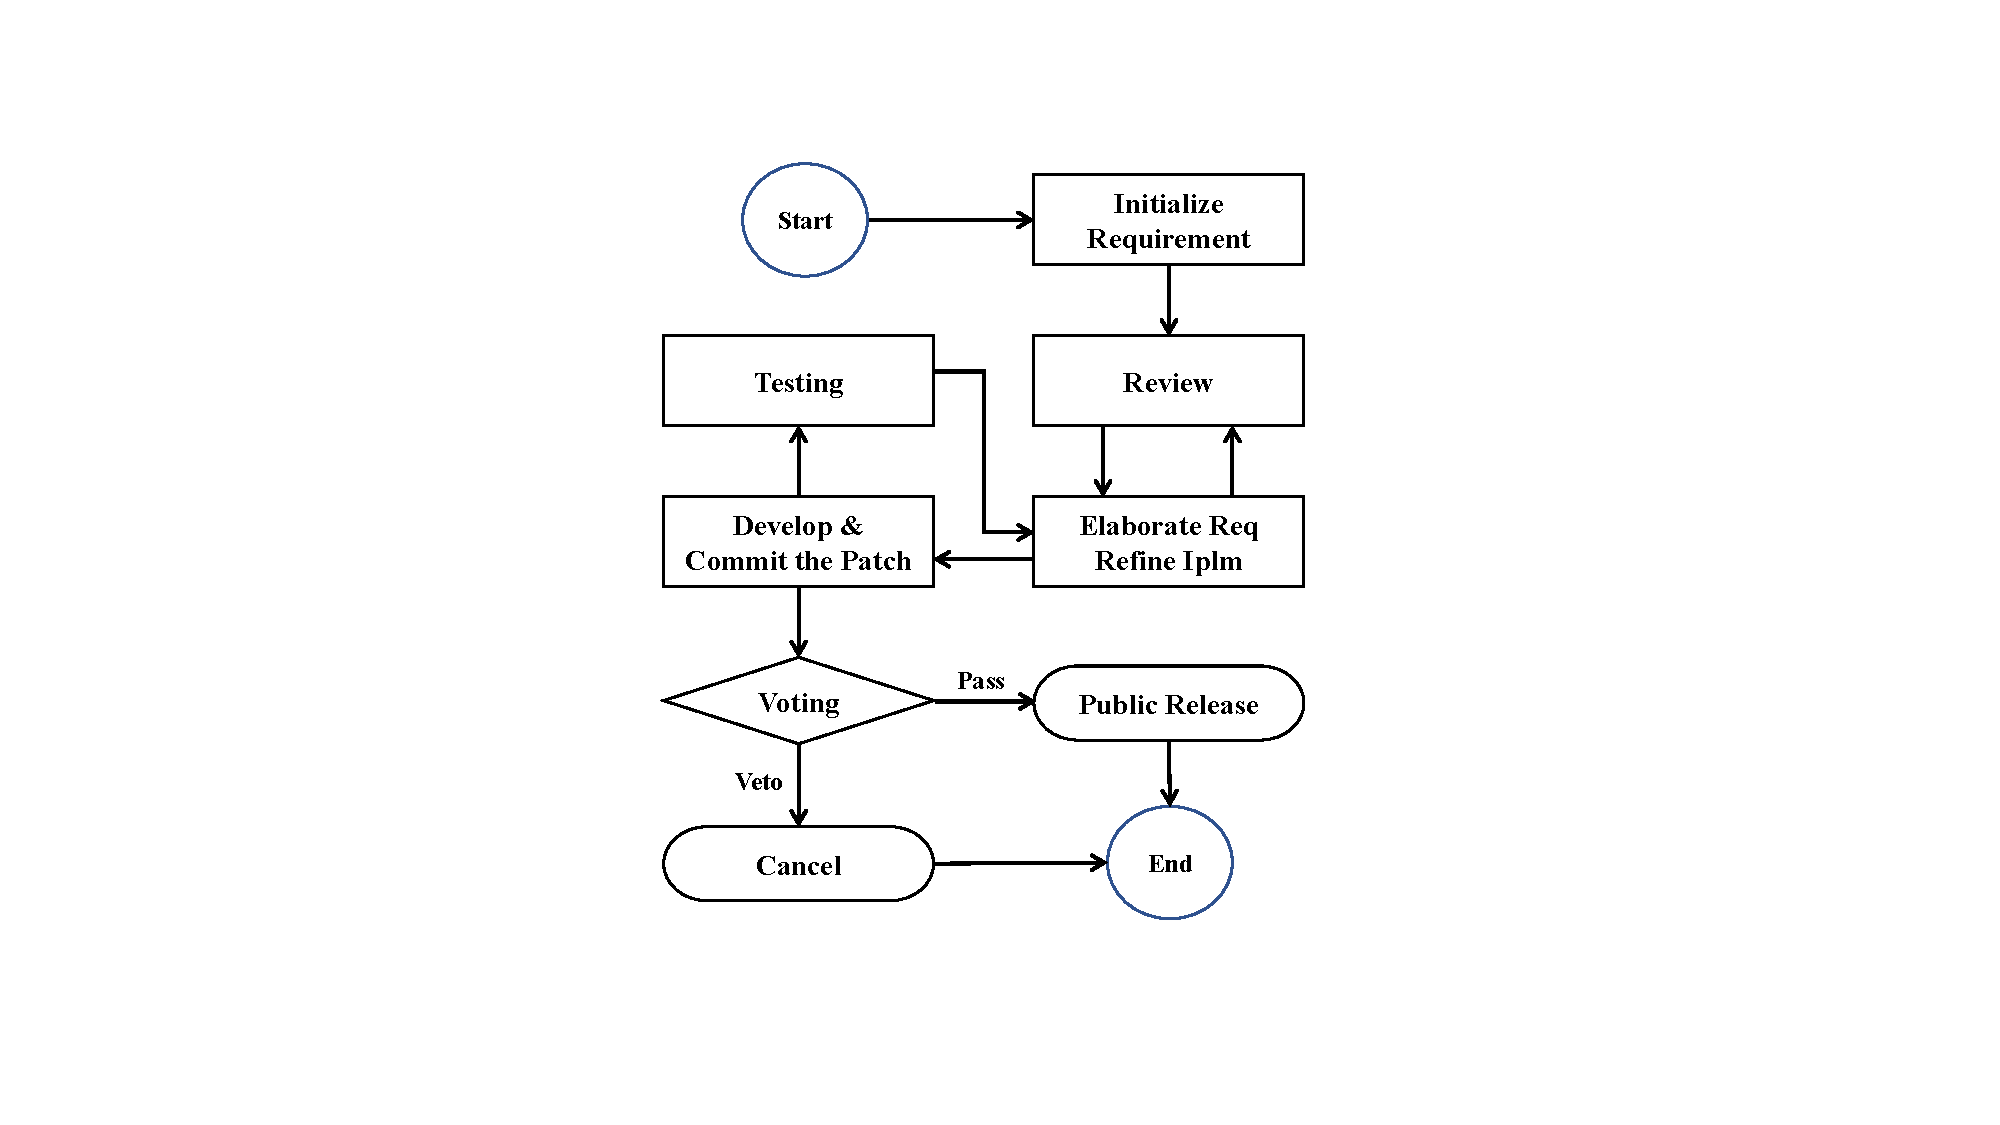
\includegraphics[page=1, width=.85\columnwidth]{jit.pdf}
	\caption{Refinement and Resolution of just-in-time Requirements.}
	\label{JIT}
\end{figure}

This section presents the JIT RE refinement and resolution process we have explored in our study. We observe that all the studied requirements follow an iterative and evolutionary approach. Figure 1 presents the general refinement and resolution process that we find common among the requirements. Subsequently, we specify each activity in the process and then include further discussions based on our investigation.

\subsection{Refinement and Resolution Steps}
\textbf{Initialize Requirement.} As an essential part in RE activities, requirement initialization marks the inception of JIT requirements. For each requirement, one authorized developer (called reporter) creates a high-level feature request in the issue tracking system with a short and clear title. In addition, the reporter provides a brief description to guarantee that all other developers have an original idea about the requirement specification before moving forward to the review activity.

\textbf{Review.} The review takes place after the requirement is reported. This activity includes two courses of action.

\textit{Requirement Review}: When the requirement is proposed, there is an informal review to verify if the requirement is eligible for implementation. In FIREFOX-480148, for example, one participant argues that this feature had been implemented before and should not be integrated into the current system (this claim, however, is later disproved). If the requirement passes through verification,  others can contribute to further elaboration, making it fit for the project roadmap.

\textit{Implementation Review}: Whenever a developer commits a patch, he/she notifies others by posting a comment over the issue tracking system. The contributors download committed patch to their local machines, examine and run the code for further testing and review. By doing so, other developers gain crucial insights into the committed patch and provide constructive feedback for improvement, if necessary.

Beside above reviews, each project might have exclusive standards to examine the qualification of the requirement and its associated implementation. In Firefox, for instance, patches that are module-crossed, have a high impact on the existing system, or are likely to involve security aspects, will have to undergo an additional super-review that consists of crucial expert-reviews for critical standards.

\textbf{Elaborate Requirement / Refine Implementation.} We notice in our study that JIT requirements and their associated implementation are highly coupled. Usually, JIT requirements are not well-defined upfront before implementation begins. Therefore, some misconceptions naturally exist during implementation. The following are some typical problems the developers addresses in the JIT requirements we examine. 

\textit{Requirement Elaboration}: At first, a JIT requirement is stated as a compact title with a short description. Unsurprisingly, reporters sometimes have difficulties anticipating all suitable uses for the users. Hence, there might be some unpleasant user experiences when the feature is developed at the beginning. For instance, in MYLYN-256699, users can only trigger editing description by double-clicking on the text field. This approach seemed inappropriate where several developers pointed out that the common practice should be one-click when setting cursor whereas double-click is used for selecting text. As a result, the developer changed to one-click editing and everyone came to an agreement. We identify that the refined requirement specification gradually reaches consensus and fulfills project roadmap in this manner.

\textit{Implementation Refinement}: Implementation plays an important role in allowing a JIT requirement to be integrated into the system. For all three projects, quality code is found to be absolutely crucial. For each committed patch, developers examine the code, identify potential flaws, if any, and provide suggestions to improve the current implementation. The main aspects that developers focus on to refine the implementation are: (1) \textbf{Correctness}: the implementation works the way specification states (e.g., LUCENE-2127, MYLYN-256699); (2) \textbf{ Performance}: the implementation operates efficiently (e.g., LUCENE-2127, MYLYN-116487); and (3) \textbf{Coding Style}: the implementation follows the coding rules specified for a certain project (e.g., FIREFOX-767676, FIREFOX-480148).

As we notice in our study, this activity has a strong relationship with other activities. A development loop among Testing, Review, Elaboration, and Development activities is established to construct an effective and well-defined JIT requirement. During the interaction among these activities, JIT requirements and their implementation progress gradually.

\textbf{Develop and Commit the Patch.} In this activity, the developer basically transforms his understanding about the requirement specification, which is shaped through his own experience and others' feedback, to code and subsequently pushes the changes to the remote repository. The original reporter plays a vital role in developing the code. However, following the nature of OSS projects, other developers are also considerably involved in the activity. During the discussion, remaining developers can either give valuable suggestions (e.g., LUCENE-2127) or develop their own implementation and commit to the development repository (e.g., MYLYN-256699). As the requirement becomes more mature, the implementation also progresses to adapt with constructive feedback from reviewers.
 
\textbf{Testing.} The testing activity takes place after a developer commits the code in order to examine the implementation and provide helpful feedback. It includes but not limited to:
\begin{itemize}
	\item Functionality Testing - justify that the new feature operates in an expected manner (all the studied requirements)
	\item GUI Testing - make sure that the GUI is consistent with the existing system and the design elements display in an expected manner (e.g., MYLYN-256699)
	\item Performance Testing - verify the efficiency of the system with the new implementation (e.g., LUCENE-2127)
	\item System Consistency Testing - verify that the newly implemented feature follows and utilizes existing system designs (all the studied requirements)
\end{itemize}

\textbf{Voting.} After finalizing the requirement specification and implementation, one last step is conducted to decide if the patch should be released to public or not. The voting process can take place over IRC, on mailing lists,  or even in issue comments. For example, in LUCENE, an email is sent with a subject starting with \textbf{[VOTE]} to the mailing list calling for a vote. If all members vote for it, the patch will be integrated into the released version. Otherwise, if any member objects the patch, he/she needs to deliver convincing reasons and must provide an alternative implementation (as stated in the Apache Foundation Software website). The substitution will then be reviewed and examined for its feasibility. If passed, a new issue will be created triggering the lifecycle of a new requirement.

We, however, did not observe any replacement for the JIT requirements we studied. One underlying rationale we observe is that most of the developers involved in the feature already participated in the discussion over the issue tracking systems. They examined the feasibility of the feature and provided feedback. That resulted in a mature fully-developed specification, making consensus in the voting  process inevitable. 

\section{Discussion}
While conducting this preliminary research, we have discovered encouraging insights about the activities that drive the development of JIT requirements, thereby leading to the refinement process we have presented in this paper. This is a generalized process intended to be applicable beyond the six functional and non-functional JIT requirements we have studied. We notice a significant association among activities that gradually shapes a complete JIT requirement.

Research on JIT requirements is at the early of its dawn and this study aims to further expand understanding about the JIT aspects. Nonetheless, due to limited scope of this paper, the number of JIT requirements studied is yet very small. The critical sampling technique~\cite{patton} has been used to seek for interesting patterns of functional and non-function JIT requirements. However, our number is constrained compared to the substantial amount of requirements our studied projects possess. In addition, with the studied non-functional JIT requirements, we notice that the developers mainly focus on implementation refinement rather than requirement elaboration (e.g., FIREFOX-767676, LUCENE-2127, MYLYN-116487). It should be noted that we have chosen non-functional requirements with a variety of focus, including security, performance and testability, so that the observation is broadly generalized. Such observation inspires us to formulate following questions regarding JIT requirements and our refinement process.
\begin{itemize}
\item \textit{Q1}: How general the refinement process is? Is it possible to apply this process to a variety of JIT requirements?
% both in terms of functional and non-functional?
\item \textit{Q2}: Do the quality of JIT requirements really improved if they follow the refinement process?
\item \textit{Q3}: Is there any distinction between the elaboration processes of functional and non-functional JIT requirements?
%Do non-functional JIT requirements strictly follow the refinement process or their refinement process focus only on certain activities?
\end{itemize} 

\section{Limitation and future work}
In this case study, we have analyzed the refinement and resolution of both functional and non-functional JIT requirements in three large OSS systems. We showed how JIT requirements evolve through a set of activities with the supportive collaboration from developers in OSS communities. In addition, we formulated three questions that could open subsequent research avenues in JIT RE. Our findings, however, are based on two requirements from each of three subject systems, which is a major limitation. We plan further comprehensive studies to strengthen our results and address the aforementioned research questions.

\section*{References}

\bibliography{citation}

\end{document}